\documentclass[12pt, a4paper]{article}

\usepackage[utf8]{inputenc}
\usepackage[russian]{babel}
\usepackage{geometry}
\usepackage{mathtools}
\usepackage{verbatim}
\usepackage{indentfirst}
\usepackage{caption}
\usepackage{subcaption}
\usepackage{import}
\usepackage{xifthen}
\usepackage{pdfpages}
\usepackage{transparent}
\usepackage{graphicx}
\usepackage{caption}
\usepackage{hyperref}
\usepackage{float}

\newcommand{\norm}[1]{\lVert #1 \rVert}
\newcommand{\abs}[1]{\lvert #1 \rvert}
\usepackage[oglav,spisok,boldsect,eqwhole,figwhole,hyperref,hyperprint,remarks,greekit]{./style/fn2kursstyle}

\graphicspath{{./style/}{./figures/}}

\frenchspacing

\title{Прямые методы решения систем
	линейных алгебраических уравнений}
\lab{1}
\author{М.\,А.~Каган}
\creator{И.\,А.~Яковлев}
\supervisor{}
\group{ФН2-51Б}
\date{2024}

\begin{document}
	\maketitle
	\tableofcontents
	
	\newpage
	
	\section{Исходные данные}
	
	Система линейных уравнений №1:
	\[
	\left \{ \begin{array}{ccccccccc}
		0.2910 x_1  & +   &   1.8100 x_2 & +   &     9.3110 x_3 & +    &    9.1100 x_4 & = & 4.2280\\
		1.4500  x_1 & + &     8.5790 x_2 & +  &     44.1950 x_3  & +  &    42.9950 x_4  & = & 20.4290\\
		-0.2900 x_1  & - &     1.7980 x_2 & - &      9.2500 x_3   & - &    9.0500 x_4 & = & -4.2080  \\
		0.0000  x_1  & + &     0.0820 x_2  & +  &     0.4100 x_3 & +  &      0.4500 x_4 & = & 0.1220
	\end{array}	\right.
	\]
	 
	Система линейных уравнений №2:
	 \[
	 \left \{ \begin{array}{ccccccccc}
	 -106.4000 x_1 & - & 7.0000 x_2 & - & 4.9900 x_3 & + & 0.2600 x_4 & = & 1040.8100\\
	3.6100 x_1 & + & 22.2000 x_2 & - & 8.5900 x_3 & - & 8.9200 x_4 & = & 615.4100 \\
	 2.2800 x_1 & + & 7.7500 x_2 & + & 52.2000 x_3 & + & 9.6500 x_4 & = & 427.5400 \\
	 -9.0000 x_1 & + & 5.8100 x_2 & - & 0.0900 x_3 & + & 136.8000 x_4 & = & -265.3500
	\end{array}	\right.
	 \]  
	\section{Краткие сведения}
	Пусть $A$ --- невырожденная матрица $n \times n$, $b$ --- ненулевой n-мерный вектор. Необходимо найти такой n-мерный вектор $x$, чтобы он удовлетворял уравнению
	\begin{equation}
		\label{eq}
		A x = b.
	\end{equation}
  
	\subsection{Алгоритм Гаусса}
	
	Метод Гаусса заключается в последовательном обнулении элементов, находящихся под главной диагональю матрицы $A$ (приведение системы к верхнетреугольному виду), и последовательное вычисление элементов неизвестного вектора $x$ решением линейных уравнений. Вычисление элементов матрицы происходит по формуле $a^{(k)}_{ij} = a^{(k-1)}_{ij} - c_{ik} a^{(k-1)}_{kj}$, где $k$ - номер итерации, $c_{ik} = a^{(k)}_{ik} \, / \, a^{(k)}_{kk}$.
	
	\subsection{Метод QR-разложения}
		Метод QR-разложения заключается в том, чтобы матрицу $A$ представить как произведение ортогональной матрицы $Q$ и верхней треугольной матрицы $R$.
		
		Рассмотрим алгоритм метод вращений, для нахождения матрицы $T=Q^{\text{T}}$:
		пусть $T_{i \, j}$ --- матрица $n \times n$ вида :
		\[
		T_{i \, j}(A) = \begin{pmatrix}
			1 & 0 & \hdotsfor{5} &  0 \\
			0 & 1 & \hdotsfor{5} &  0 \\
			\hdotsfor{8} \\
			0 & 0 & \ldots & c & \ldots & s & \ldots &  0 \\
			\hdotsfor{8}  \\
			0 & 0 & \ldots & -s & \ldots & c & \ldots &  0 \\
			\hdotsfor{8}  \\
			0 & 0 & \hdotsfor{5} &  1 \\
		\end{pmatrix}\!, \;\;\; \text{где} \; 1 \le i < j \le n.
		\]
		Коэффициенты $c$ и $s$ вычисляются по следующим формулам:
		
		\[
		\begin{array}{cc}
			c = \cfrac{a_{i \, i}}{\sqrt{ a_{i \, i}^2 + a_{j \, i}^2}}\, , & s = \cfrac{a_{i \, j}}{\sqrt{ a_{i \, i}^2 + a_{j \, i}^2}},
		\end{array}
		\]
		При умножении $T_{i \, j}(A) \cdot  A = A^{(1)}$ элемент $a^{(1)}_{j \, i}$ равняется нулю, следовательно
		 \[
		 T = T_{n - 1 \, n} \cdot \ldots \cdot T_{2 \, 4} T_{2 \, 3} T_{1 \, n} \ldots \cdot T_{1 \, 3}T_{1 \, 2}.
		 \]
		 где $T_{i \, j} = T_{i \, j}(A^{(l)}), \; l = (i - 1) n + j - i$, а верхняя треугольная матрица $R = T A$. Таким образом, уравнение (\ref{eq}) сводится к двум более простым уравнениям:
		 \[
		 \begin{cases}
		 	R x = b^*, \\
		 	Q b^* = b.
		 \end{cases}
		 \]
		 
		 
		 
		
		
		
	% \section{Ход работы}
	% \subsection{Исходные данные}
	% \subsection{Результаты расчетов}
	% \subsection{Анализ результатов}
	
	\section-{Контрольные вопросы}
	\begin{enumerate}
		\item \textbf{Каковы условия применимости метода Гаусса без выбора и с выбором ведущего элемента?}
		
		\textit{\textbf{Ответ:}}
		
		Метод Гаусса без выбора ведущего элемента может быть применен только в том случае, если в процессе преобразования невырожденной матрицы, на главной диагонали не возникает нулевых элементов, поскольку данный алгоритм предполагает деление на элементы $a^{(i-1)}_{i\,i}$, где $i = 1, \ldots , n - 1$. Таким образом, чтобы расширить класс матриц, над которым применим метод Гаусса, достаточно предварительно <<выбирать>> неизвестное с ненулевым коэффициентом. Выбор происходит посредством перестановок строк и столбцов матрицы.
		
		\textbf{\item Докажите, что если $\det A \neq 0$, то при выборе главного элемента в столбце среди элементов, лежащих не выше главной диагонали, всегда найдется хотя бы один элемент, отличный от нуля.}
		
		\vspace*{0.2cm}
		\textit{\textbf{Ответ:}}
		
		Пусть при выборе главного элемента в одном из столбцов среди элементов, лежащих не выше главной диагонали нет ни одного отличного от нуля элемента. Тогда, после приведения матрицы к верхнетреугольному виду, определитель матрицы $\det A$ будет равен произведению элементов на главной диагонали; так как один из элементов равен нулю, $\det A = 0$, что противоречит исходному предположению.
		
		\textbf{\item В методе Гаусса с полным выбором ведущего элемента приходится не только переставлять уравнения, но и менять нумерацию неизвестных. Предложите алгоритм, позволяющий восстановить первоначальный порядок неизвестных.}
		
		\vspace*{0.2cm}
		\textit{\textbf{Ответ:}}
		
			Чтобы восстановить изначальный порядок неизвестных, можно хранить их индексы в отдельном массиве, каждый раз меняя их местами вместе со столбцами. При окончании работы алгоритма необходимо отсортировать решение по переставленным индексам. 
		
	\textbf{	\item Оцените количество арифметических операций, требуемых для QR-разложения проивзольной матрицы $A$ размера $n \times n$.}
		
		\vspace*{0.2cm}
		\textit{\textbf{Ответ:}}
		
			Для вычисления констант $c$ и $s$ необходимо произвести минимум две операции умножения и две операции деления. Для умножения матрицы $A$ на матрицу $T_{i \, j}$ достаточно заменить строки $i$ и $j$ на их линейные комбинации, для чего требуется умножить каждый элемент i-й и j-й строки сначала на $c$ и $s$, затем на $-s$ и $c$ соответственно: в сумме получается $4n$ операции. Для приведения матрицы $A$ к верхнему треугольному виду необходимо обнулить $\frac{1}{2}n(n-1)$ элементов, а для обнуления одного элемента необходимо произвести $4n + 4$ операций, следовательно в сумме получается $2n(n + 1)(n - 1)$ операций. Для решения полученной системы необходимо произвести еще приблизительно $n(n - 1)$ операций. В конечном итоге получаем: $2 n^3 + n^2 - 3 n \sim 2 n^3$.
		
		\textbf{\item Что такое число обусловленности и что оно характеризует? Имеется ли связь между обусловленностью и величиной определителя матрицы? Как влияет выбор нормы матрицы на оценку числа обусловленности?}
		
		
		
		\vspace*{0.2cm}
		\textit{\textbf{Ответ:}}
		\begin{enumerate}
		\item Рассмотрим линейную систему уравнений заданных с погрешностью:
		\[
		A(x + \varDelta x) = b + \varDelta b.
		\]
		Оценим погрешности $\varDelta x$ и $\varDelta b$:
		\begin{equation}
			\label{obuslov}
			\norm{\varDelta x} \le \norm{A^{-1}} \norm{\varDelta b}
		\end{equation}
		Теперь поделим на $\norm{x}$ и $\frac{\norm{b}}{\norm{A}}$ левую и правую часть соответственно:
		
		\[
			\frac{\norm{\varDelta x}}{\norm{x}} \le \norm{A}\norm{A^{-1}} \frac{\norm{\varDelta b}}{\norm{b}},
		\]
		\begin{equation}
			\label{opred-obuslov}
			\frac{\norm{\varDelta x}}{\norm{x}} \le  \frac{\norm{\varDelta b}}{\norm{b}} \, \text{cond}\, A,
		\end{equation}
		образом была получена связь между относительными погрешностями правой и левой части. Значение $\norm{A}\norm{A^{-1}}$ будем называть числом обусловленности матрицы $A$, которое характеризует насколько ошибки входных данных влияют на ошибку результата и наоборот.
		\item Между числом обусловленности и определителем матрицы нет прямой связи: с одной стороны, чем меньше $\det A$, тем больше $\det A^-{1}$, из-за чего $\norm{A^{-1}}$ также становится больше, следовательно, из оценки (\ref{obuslov}) следует большее влияние погрешностей левой части на правую. С другой стороны, если собственные значения матрицы не сильно различаются, то и значение $\text{cond}\, A$ не будет слишком велико, например, пусть матрица:
		
		\item Выбор нормы матрицы на прямую влияет на оценку числа обусловленности --- это следует из оценки (\ref{opred-obuslov}). Приведем пример: рассмотрим матрицу
		\[
		A = \begin{pmatrix}
			0 & 100 & 0\\
			34 & 34 & 34 \\
			1 & 0 & 0
		\end{pmatrix}, \; \; \; \; A^{-1} = \begin{pmatrix}
		0 & 0 & 1\\
		\frac{1}{100} & 0 & 0 \\
		\frac{1}{100} & \frac{1}{34} & -1
		\end{pmatrix}.
		\]
		Тогда число обусловленности посчитанное по кубической норме будет равно $\text{cond}_\infty \, A \approx 106$, а по октаэдрической норме будет равно $\text{cond}_1 \, A \approx 268$, т.е. разница больше чем в два раза.
		
		
		\end{enumerate}
		
		
		
		\textbf{\item Как упрощается оценка числа обусловленности, если матрица является:
			\begin{enumerate}
				\item диагональной;
				\item симметричной;
				\item ортогональной;
				\item положительно определенной;
				\item треугольной;
			\end{enumerate}}
		
		\vspace*{0.2cm}
		\textit{\textbf{Ответ:}}
		
		\begin{enumerate}
			\item У диагональной матрицы $A$ собственные значения являются диагональными элементами этой матрицы $a_{ii}, 1 \leq i \leq n$. Обратная к диагональной матрице $A^{-1}$ тоже является диагональной, причем её диагональными элементами будут $\frac{1}{a_{ii}}, 1 \leq i \leq n$; тогда число обусловленности 
			\begin{equation*}
				cond A \geq \frac{ \max\limits_{1 \leq i \leq n} \lvert a_{ii}\rvert }{\min\limits_{1 \leq i \leq n} \lvert a_{ii} \rvert}.
			\end{equation*}
			
			\item Для вычисления числа обусловленности необходимо вычислить нормы матрицы $\lVert {A} \rVert$ и $\lVert A^{-1} \rVert$; ввиду симметрии, требуемые для нахождения норм $\norm{A}_{\infty} = \max\limits_i \sum\limits_{j=1}^n \abs{a_{ij}}$, $\norm{A}_1 = \max\limits_j \sum\limits_{i=1}^n \abs{a_{ij}}$ и $ \norm{A}_2 = \Bigl ( \sum\limits_{i,j=1}^{n} a_{ij}^2 \Bigr)^{1/2}$ вычисления будут в половину раз проще.
			
			\item Ортогональная матрица $A$ имеет следующее свойство: $A^T A= E$, где $E$ -- единичная матрица. Таким образом, $A^{-1} = A^T$, и её число обусловленности $\text{cond} A \geq \norm{A} \norm{A^{-1}} = \norm{A} \norm{A^{T}}$, что упрощает вычисления.
			
			\item Положительно определенная матрица имеет все собственные значения положительные, что позволяет получить оценку для числа обусловленности через их соотношение:
			\begin{equation*}
				\text{cond} A = \frac{\lambda_{max}}{\lambda_{min}}.
			\end{equation*}
			
			\item Для треугольной матрицы (верхней или нижней) оценку числа обусловленности также можно получить через её диагональные элементы, так как собственные значения треугольной матрицы находятся на её диагонали:
			\begin{equation*}
				\text{cond} A = \frac{\max {\abs{\lambda_i}}}{ \min \abs{{\lambda_i}} }.
			\end{equation*}
			
			
		\end{enumerate}
		
		\textbf{\item Применимо ли понятие числа обусловленности к вырожденным матрицам?}
		
		\vspace*{0.2cm}
		\textit{\textbf{Ответ:}}
		
		Нет, поскольку по определению обусловленности: 
		\[
		\text{cond} A = \norm{A} \norm{A^{-1}},
		\]
		то есть обязана существовать обратная матрица.
		
		\textbf{\item В каких случаях целесообразно использовать метод Гаусса, а в каких -- методы, основанные на факторизации матрицы?}
		
		\vspace*{0.2cm}
		\textit{\textbf{Ответ:}}
		
		Методы разложения требуют значительно больше операций, чем метод Гаусса, однако их удобно использовать, если требуется решить большое количество уравнений с одной и той же матрицей, более того, такие вычисления будут более устойчивы, то есть их можно использовать для плохо обусловленных матриц.
		
		\textbf{\item Как можно объединить в одну процедуру прямой и обратный ход метода \mbox{Гаусса}? В чем достоинства и недостатки такого подхода?}
		
		\vspace*{0.2cm}
		\textit{\textbf{Ответ:}}
		
		 Прямой ход метода \mbox{Гаусса} находит верхнюю треугольную матрицу $U$ для некоторой квадратной матрицы $A$. Следовательно, если использовать алгоритм над транспонированной матрицей $A^\text{T}$, то он найдет нижнюю треугольную матрицу $L$ для матрицы $A$. Таким образом, для полноценной реализации метода Гаусса достаточно дважды запустить процедуру прямого хода: сначала для матрицы $A$, затем для матрицы $U^\text{T}$. При таком подходе в разы упрощается реализация метода Гаусса, при этом происходит повторный проход по нулевым элементам матрицы $U^\text{T}$ и возникает необходимость в транспонировании~$U$, что может существенно увеличить время исполнения алгоритма .  
		
		\textbf{\item Объясните, почему, говоря о векторах, норму $ \norm{\cdot}_1 $ часто называют октаэдрической, норму $ \norm{\cdot}_2 $ -- шаровой, а норму $ \norm{\cdot}_{\infty} $ -- кубической.}
		
		\vspace*{0.2cm}
		\textit{\textbf{Ответ:}}
		
		Кубическая норма $ \norm{x}_{\infty} = \max\limits_k \abs{x_k}$ называется так потому, что множество $ \norm{x}_{\infty} \leq 1$ представляет собой куб со стороной длиной 2. Аналогично, для октаэдрической нормы $ \norm{x}_{1} = \sum\limits_{j=1}^n \abs{x_i}$ множество $ \norm{x}_{1} \leq 1 $ представляет собой октаэдр, а для евклидовой (шаровой) нормы $ \norm{x}_{2} = \Bigl ( \sum\limits_{i=1}^{n} x_i^2 \Bigr)^{1/2} $ множество $ \norm{x}_{2} \leq 1 $ -- шар радиусом 1 в декартовых координатах.
		
	\end{enumerate}
	
		\newpage
	\section-{Дополнительные вопросы}
	
	\begin{enumerate}
		\item \textbf{Посчитать ${\det A \; \text{при} \; n = 4}$ через миноры.}
		
		\vspace*{0.2cm}
		\textit{\textbf{Ответ:}}
		
		Пусть дана матрица $A$:
		\begin{equation*}
			A = 
			\begin{pmatrix}
				a_{11}& a_{12}& a_{13}& a_{14}\\
				a_{21}& a_{22}& a_{23}& a_{24}\\
				a_{31}& a_{32}& a_{33}& a_{34}\\
				a_{41}& a_{42}& a_{43}& a_{44}
			\end{pmatrix}
			.
		\end{equation*}
		Вычислить определитель этой матрицы можно вычислить с помощью разложения по строке или столбцу. Запишем разложение по первой строке:
		\begin{multline*}
			\det A = a_{11} \cdot
			\begin{vmatrix}
				a_{22}& a_{23}& a_{24}\\
				a_{32}& a_{33}& a_{34}\\
				a_{42}& a_{43}& a_{44}
			\end{vmatrix}
			- a_{12} \cdot
			\begin{vmatrix}
				a_{21}& a_{23}& a_{24}\\
				a_{31}& a_{33}& a_{34}\\
				a_{41}& a_{43}& a_{44}
			\end{vmatrix}
			+\\
			+ a_{13} \cdot 
			\begin{vmatrix}
				a_{21}& a_{22}& a_{24}\\
				a_{31}& a_{32}& a_{34}\\
				a_{41}& a_{42}& a_{44}
			\end{vmatrix}
			- a_{14} \cdot
			\begin{vmatrix}
				a_{21}& a_{22}& a_{23}\\
				a_{31}& a_{32}& a_{33}\\
				a_{41}& a_{42}& a_{43}
			\end{vmatrix}
			.
		\end{multline*}
		
		\textbf{\item Расписать вопрос №3 более подробно: привести пример (небольшой порядок).}
		
		\vspace*{0.2cm}
		\textit{\textbf{Ответ:}}
		
		Пусть дана система уравнений (1):
		\begin{equation}
			\begin{cases}
				x_1 + 5 x_2 + 3 x_3 = 8;\\
				3 x_1 + x_2 + 8 x_3 = 3;\\
				6 x_1 + 2 x_2 + x_3 = 16.
			\end{cases}
		\end{equation}
		Матрицы $A$ и $b$ соответственно:
		\begin{equation*}
			\begin{aligned}
				&A  = 
				\begin{pmatrix}
					1&5&3\\
					3&1&8\\
					6&2&1
				\end{pmatrix}
				, &b = 
				\begin{pmatrix}
					8\\3\\16
				\end{pmatrix}
				.
			\end{aligned}
		\end{equation*}
		Создадим два массива перестановок, для строк и для столбцов:
		\begin{equation*}
			\begin{aligned}
				&\text{rows}_{str} = \bigl(1, \, 2, \,3 \bigr),
				&\text{rows}_{col} = \bigl(1, \, 2,  \,3 \bigr).
			\end{aligned}
		\end{equation*}
		Главным элементом для позиции (1, 1) будет элемент $A_{2\, 3}$. Сделаем соответствующую перестановку строк и столбцов:
		\begin{equation*}
			\begin{aligned}
				&A^{new} = 
				\begin{pmatrix}
					8&1&3\\
					3&5&1\\
					1&2&6
				\end{pmatrix}
				, &b^{new} = 
				\begin{pmatrix}
					3\\8\\16
				\end{pmatrix},
			\end{aligned}
		\end{equation*}
		массивы перестановок при этом имеют вид:
		\begin{equation*}
			\begin{aligned}
				&rows_{str}= \bigl[3, \, 2, \, 1 \bigr], &rows_{col} = \bigl[2, \, 1, \,3 \bigr].
			\end{aligned}
		\end{equation*}
		При окончании работы алгоритма с помощью данных массивов можно восстановить исходный порядок переменных и строк в матрице $A$.
		
		\textbf{\item Число обусловленности $\text{cond}A = 100$. Хорошо или плохо?}
		
		\vspace*{0.2cm}
		\textit{\textbf{Ответ:}}
		
		Число обусловленности $\text{cond}A$ матрицы $A$ связано с оценкой того, как ошибка в входных данных $\delta b$ влияет на ошибку в решении $\delta x$ системы уравнений $Ax = b$:
		\begin{equation*}
			\frac{\norm{\delta x}}{\norm{x}} \leq \text{cond} A \cdot \frac{\norm{\delta b}}{\norm{b}}.
		\end{equation*}
		Скажем, если число обусловленности равна $100$, то и ошибка может быть увеличена в 100 раз, и в различных задачах это будет иметь разную степень приемлемости, которая, в частности, будет зависеть от ошибки входных данных~$b$.  Например, если ошибка составляет $0.001$, т.е. $\frac{\norm{\delta b}}{\norm{b}} = 0.001$, то верхняя оценка для ошибки в решении будет:
		\begin{equation*}
			\frac{\norm{\delta x}}{\norm{x}} \leq 100 \cdot 0.001 = 0.1.
		\end{equation*}
		
		\textbf{\item Посчитать число операций в методе Гаусса и сравнить с числом операций QR-алгоритма.}
		
		\vspace*{0.2cm}
		\textit{\textbf{Ответ:}}
		
		Деление вектора $b$ на главный элемент строки -- n операций, деление элементов строки на главный элемент строки -- $\frac{n(n-1)}{2}$ операций, вычитание из вектора $b$ одной из предыдущих строк, умноженной на главный элемент текущей строки -- $\frac{n(n-1)}{2}$ операций, вычисление остальных коэффициентов матрицы -- сумма квадратов от 1 до $n-1$, $\frac{1}{6} \left(n-1\right) n \left( 2n - 1 \right)$ операций, обратный ход -- $\frac{n(n-1)}{2}$ операций. Итого:
		\[
		n + 3 \frac{n(n-1)}{2} + \frac{1}{6} \left(n-1\right) n \left( 2n - 1 \right) = \frac{n}{3} \left(n^2 + 3n - 1 \right) \sim \frac{n^3}{3}.
		\]  
		
		Таким образом, метод Гаусса в среднем работает приблизительно в 6 раз быстрее, чем метод QR-разложения. 
	\textbf{\item Количество операций в методе Гаусса с полным выбором элемента.}
	
	\vspace*{0.2cm}
	\textit{\textbf{Ответ:}}
	
	К прямому и обратному ходу в классическом методе Гаусса добавляется поиск максимального элемента и перестановка строк и столбцов на каждой итерации.
	
	Поиск максимального элемента: на каждом шаге поиск происходит по $(n - k + 1) \times (n - k + 1)$ 
	элементам, $k = \overline{1, \, n-1}$. Количество операций -- сумма квадратов от 1 до $n - 1$, равная $\frac{1}{6} \left(n-1\right) n \left( 2n - 1 \right)$.
	
	Перестановка строк и столбцов - $O(n)$ операций на каждом шаге, то есть за $n-1$ шагов потребуется приблизительно $n^2$ операций.
	
	При добавлении данных операций к классическому методу Гаусса, общее количество операций оценивается как $\frac{2n^3}{3}$, что есть в два раза больше, чем в классическом методе.
	
	\textbf{\item Нарисовать картинки к 10 вопросу, определение эквивалентных норм.}
	
	\vspace*{0.2cm}
	\textit{\textbf{Ответ:}}
	
	\begin{figure}[H]
		\begin{minipage}[b]{0.45\linewidth}
			\centering
			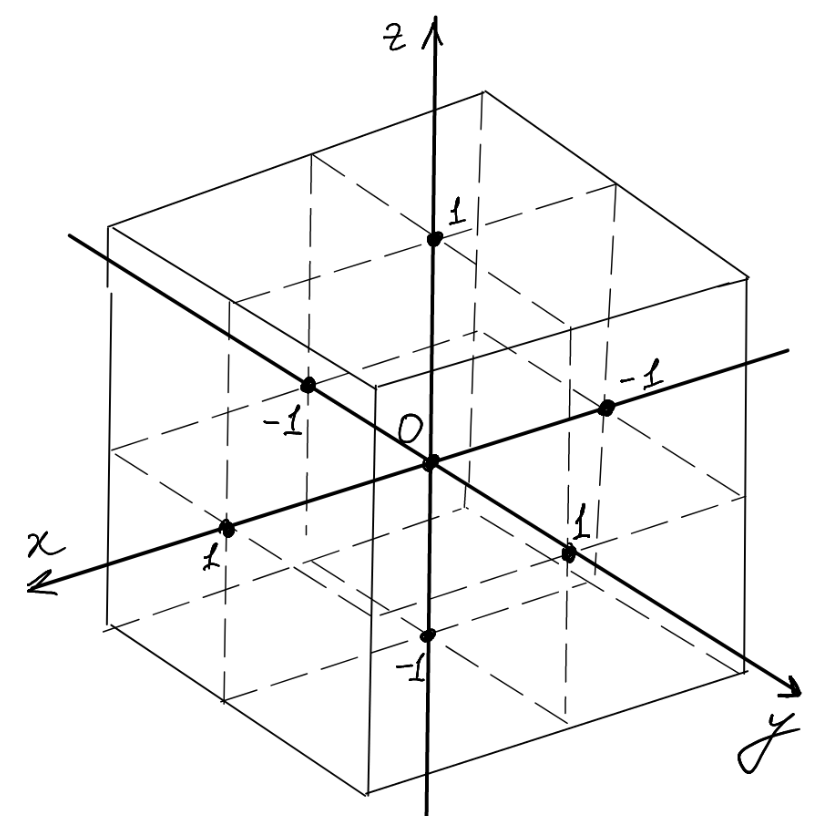
\includegraphics[width=0.7\linewidth]{pic1.png}
			\caption{Множество $\norm{x}_{\infty} \leq 1$}
			\label{rrr}
		\end{minipage}
		\hfill
		\begin{minipage}[b]{0.45\linewidth}
			\centering
			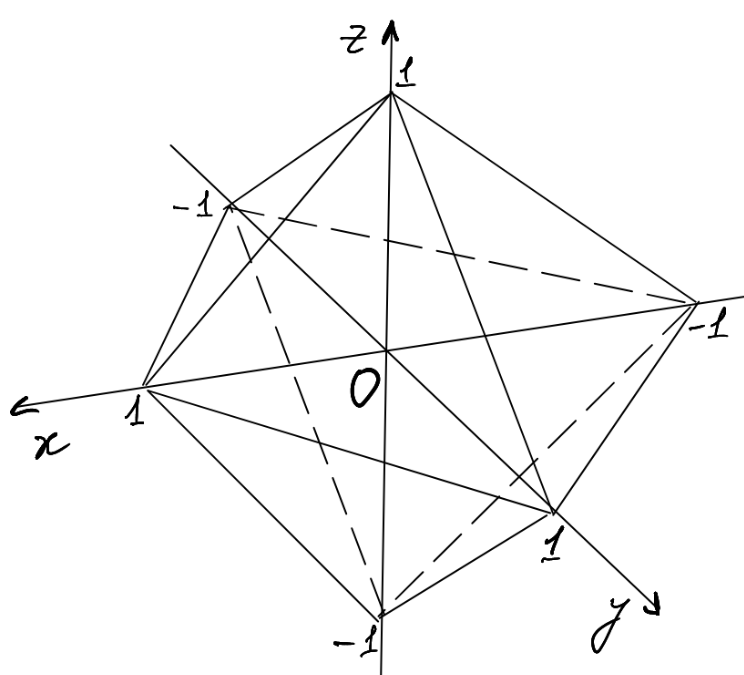
\includegraphics[width=0.7\linewidth]{pic2.png}
			\caption{Множество $\norm{x}_{1} \leq 1$}
			\label{ttt}
		\end{minipage}
		
		\vspace{1em}
		\begin{minipage}{\linewidth}
			\centering
			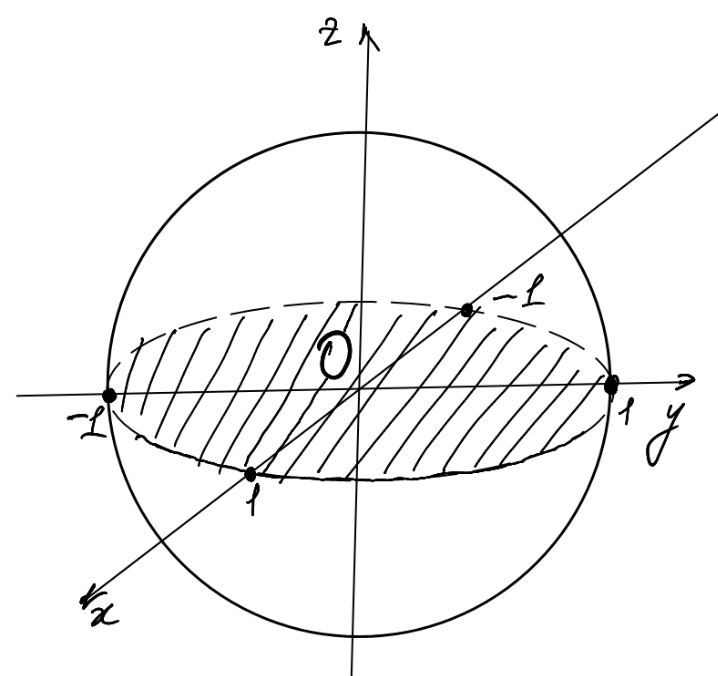
\includegraphics[width=0.3\linewidth]{pic3.png}
			\caption{Множество $\norm{x}_{2} \leq 1$}
		\end{minipage}
	\end{figure}
	
	\textbf{Определение.} Пусть $\norm{\cdot}_a$ и $\norm{\cdot}_b$ -- нормы на векторном пространстве $V$, тогда они называются \textbf{эквивалентными}, если $\exists$ положительные постоянные $C_1 > 0$ и $C_2 > 0$ такие, что для всех векторов $v \in V$ выполнены неравенства:
	\begin{equation*}
		C_1 \norm{v}_a \leq \norm{v}_b \leq C_2 \norm{v}_a.
	\end{equation*}
	
	\clearpage
	\end{enumerate}
	
\end{document}